\documentclass[12pt, algo]{cours}

\usepackage{pgf-umlcd}  % pour le diagramme des classes

\title{\textbf{\textsc{Ergo -- rapport}}}

\author{Delay Emmanuel-- Desforêts Nicolas}
\date{\today}

\parindent 0.5cm

%\makeatletter
%\renewcommand{\maketitle}{%
%  \thispagestyle{plain}
%  \begin{center}%
%  \let \footnote \thanks
%    {\LARGE \@title \par}%
%    \vskip 1.5em%
%    {\large \@author}%
%  \end{center}%
%  \par
%  \vskip 1.5em}
%\makeatother

% a3_landascape environment
\newenvironment{a3_landscape}
    {\clearpage
    \pdfpagewidth=2\pdfpagewidth
    \hsize=2\hsize
    \textwidth=2\textwidth
    \headwidth=\textwidth}
    {\newpage
    \pdfpagewidth=.5\pdfpagewidth
    \hsize=.5\hsize
    \textwidth=.5\textwidth
    \headwidth=\textwidth}


\begin{document}

\maketitle

\tableofcontents

\parskip 5pt

\pagebreak

\section{Présentation du projet}

\subsection{Présentation du jeu}

Le point de départ est le jeu \href{https://www.catalystgamelabs.com/ergo/}{Ergo}, \og The Game of Proving You Exist!\fg. Les règles détaillées sont \href{https://www.catalystgamelabs.com/download/Ergo%20Rules%202015.pdf}{ici}.

Le jeu est composé de 55 cartes : 4 de chaque variable (A, B, C ou D), 4 de chaque opérateur (ET, OU, $\implies$), 6 cartes NON, 8 parenthèses, 3 cartes Ergo et 10 cartes particulières.

Chaque joueur (4 maximum) se voit assigné une variable (A, B, C ou D) au début du jeu. À chaque manche, les joueurs essaient collectivement de créer une preuve de leur existence tout en réfutant l'existence des autres joueurs. Au début de la manche, chaque joueur reçoit 5 cartes puis, à chaque tour, un joueur pioche deux cartes et doit jouer deux cartes (éventuellement les défausser). Lorsque une carte Ergo est jouée ou qu'il n'y a plus de carte dans la pioche la preuve est terminée. À condition qu'il n'y ait pas de paradoxe, chaque joueur dont l'existence est prouvée reçoit un nombre de points égal au nombre de cartes dans la preuve. Toutes les cartes sont ensuite mélangées et une nouvelle manche est lancée. Le premier joueur ayant 50 points gagne.

Concernant la construction de la preuve, un certain nombre de règles doivent être respectées~:
\begin{itemize}
\item la preuve doit avoir au maximum 4 lignes. Dès qu'elle atteint 4 lignes, toutes les cartes supplémentaires doivent être jouées sur une de ces lignes~;
\item chaque ligne doit être syntaxiquement correcte (deux opérateurs ou deux variables ne peuvent pas se suivre, chaque parenthèse ouvrante doit correspondre à une parenthèse fermante, \dots)~;
\item une carte peut être insérée entre deux cartes déjà posées à condition que le résultat reste syntaxiquement correct.
\end{itemize}

\subsection{Le projet}

Le but initial était de réaliser une implémentation en Python de ce jeu. Pour cela, plusieurs points semblaient à traiter, plus ou moins par ordre de difficulté croissante~:
\nopagebreak
\begin{itemize}
\item analyser une ligne de la preuve pour vérifier qu'elle est syntaxiquement correcte~;
\item coder une ligne syntaxiquement correcte sous une forme exploitable (arbre, forme conjonctive normale, forme disjonctive normale, \dots ?)~;
\item déterminer à partir du codage des 4 lignes quelles variables sont prouvées ou s'il y a une contradiction~;
\item réaliser une interface graphique avec tkinter~;
\item implémenter une fonction pour pouvoir jouer contre l'ordinateur.
\end{itemize}

Finalement, tous les points précédents ont pu être traités.

%Si on finit tout ça et qu'on a peur de s'ennuyer, on pourra toujours creuser pour améliorer la façon dont l'ordinateur joue. Au pire, on demandera à Frédéric Muller de nous prêter ses TetrisBot pour qu'ils apprennent à jouer à Ergo ;-)


\section{Organisation du travail}

\subsection{Outils utilisés}

Nous avons configuré un Rasberry Pi comme serveur pour installer redmine dessus, en nous aidant beaucoup du \href{http://juramaths.fr/redmine/projects/serveur-web-sur-un-raspberry-pi/wiki}{wiki} de Frédéric Muller (merci à lui) et des article de Linux Pratique mis à notre disposition par The Big Boss (loué soit-il).

Nous avons aussi créé un dépôt sur github : \url{https://github.com/isnpaulconstans/Ergo}

La documentation technique est générée avec Sphinx, encore grâce aux articles de GNU/Linux Magasine que notre Big Boss a eu la bonté de nous fournir (Il n'en sera jamais assez remercié \footnote{Le cirage de pompe peut-il augmenter significativement la note de ce module ?}).

Les résultats sont disponibles sur \url{http://paulconstans.ddns.info/redmine/projects/ergo} et sur \url{http://paulconstans.ddns.info/documentation/}.

\subsection{Répartition du travail}

Après quelques discutions, le travail s'est assez naturellement réparti. Emmanuel Delay s'est chargé de la partie algorithmique tandis que Nicolas Desforêts s'est occupé de l'interface graphique et de la réalisation d'une page web pour les règles du jeu. Comme nous travaillons tous les deux dans le même lycée, nous avons pu nous voir régulièrement pour faire la jointure entre nos deux parties et nous mettre d'accord sur les étapes suivantes.

\section{Solutions techniques}

\subsection{Les constantes}

Les différentes constantes pouvant être utiles dans plusieurs classes, comme le nombre de cartes de chaque type, la taille des images correspondante ou les couleurs du canvas, sont rassemblées dans une classe dédiée.

\subsection{Les modules concernant les cartes}


\subsubsection{Card}

La classe \texttt{Card} définit les différentes cartes. Chaque carte a un nom, un niveau de priorité. De nombreuses méthodes permettent de déterminer de quelle carte, ou de qelle famille de carte (lettre, opérateur, joker, \dots) il s'agit. Une méthode permet aussi de \og retourner \fg les parenthèses pour transformer un parenthèse ouvrante en parenthèse fermante et réciproquement. Comme il est parfois nécessaire de comparer deux cartes, la méthode \texttt{\_\_eq\_\_} permet de tester l'égalité de deux cartes (en comparant les noms), ou d'une carte et d'une chaîne de caractères. Les cartes pouvant aussi servir de clé dans un dictionnaire, une fonction de hachage a été implémentée par la méthode \texttt{\_\_hash\_\_}.

\subsubsection{CardList}

La classe \texttt{CardList} hérite de la classe \texttt{list} et gère les listes de cartes. Elle permet d'ajouter, modifier ou supprimer une carte de la liste. Cette classe permet de déterminer si la liste de carte est syntaxiquement correcte, et dans ce cas d'y associer son écriture en notation polonaise inversée (NPI). Un attribut \texttt{modif} permet de savoir si la liste a été modifiée depuis le dernier calcul de la NPI pour éviter de le refaire inutilement.

\subsubsection{Proof}

La classe \texttt{Proof} gère les quatre prémisses. Elle répercute les modifications (ajout, suppression, changement) aux différentes prémisses et gère leur conjonction pour déterminer la NPI associée à la preuve. Elle permet également de savoir si toutes les lettres ont été jouées (pour pouvoir éventuellement jouer une carte Ergo), et le nombre de cartes jouées (pour calculer le score correspondant). Les méthodes \texttt{insert} et \texttt{pop} ont un paramètre supplémentaire qui permet de gérer deux cas différents pour chacune :
\begin{itemize}
\item l'ajout peut provenir soit d'une nouvelle carte jouée par le joueur soit de l'annulation d'une carte Tabula Rasa qui doit être gérée différemment.
\item De même , la suppression peut soit correspondre à une carte qui vient d'être jouée, soit au jeu d'une carte Tabula Rasa.
\end{itemize}

Pour pouvoir gérer ces différents cas, on maintient une liste \texttt{currently\_added} des numéro de prémisse et index des cartes qui peuvent être modifiées, ainsi qu'un booléen indiquant si la carte correspond à un jeu \og classique \fg (une carte qui vient d'être jouée et qui peut être retirée) ou au jeu d'une carte Tabula Rasa (carte qui a été supprimée par un Tabula Rasa et qui peut être remise). Les indices de cette liste doivent être actualisés à chaque ajout ou suppression de cartes dans les prémisses pour suivre les modifications. Par exemple, si une carte est ajoutée avant une carte mémorisée, l'indice de cette dernière doit être augmenté de 1 pour refléter sa nouvelle position dans la prémisse.

\subsubsection{Deck}

La classe \texttt{Deck} hérite de \texttt{list} et gère le paquet de cartes. Elle permet de tirer un certain nombre de cartes du paquet (cinq en début de partie, et deux au début de chaque tour). Les méthodes \texttt{append} et \texttt{pop} permettent de gérer les cartes supprimées par un Tabula Rasa qui doivent être remises à la fin du paquet. La méthode \texttt{is\_finished} permet de savoir si le paquet est terminé, pour le cas échéant mettre fin au tour.

\subsection{Les modules concernant les démonstrations}

L'analyse de la preuve se fait par la classe abstraite \texttt{Demonstration}. Cette classe est concrétisée par les deux classes \texttt{ForceBrute}, qui cherche à déterminer les \og variables prouvées \fg par force brute, et \texttt{DPLL} qui utilise l'algorithme de Davis-Putnam-Logemann-Loveland. Cette dernière commence par faire appel à la classe \texttt{FCN} pour obtenir l'écriture en forme conjonctive normale de la preuve. Les algorithmes utilisés dans ces classes seront décrits dans la section suivante.

\subsection{Jeu de l'ordinateur}

\subsubsection{Ordi}

Le gestion des coups possibles se fait dans la classe \texttt{Ordi}. Cette classe contient une méthode abstraite \texttt{choix\_coups} en vue de tester différentes idées concernant les deux cartes à jouer.

Une première étape consiste, si on a au moins deux parenthèses en main, à se débrouiller pour en avoir au moins une ouvrante et une fermante. Pour simplifier la gestion des cartes Fallacy et Justification, une deuxième étape consiste à mettre en premier la carte \texttt{Justification} s'il y en a une. Enfin, on travaille avec une copie de la main dans laquelle les joker (\texttt{WildVar} et \texttt{WildOp}) sont remplacés par une lettre et un opérateur (ça ne change rien à la syntaxe). Pour retrouver les cartes qui étaient initialement des jokers, j'ai ajouté un attribut \texttt{wild} à la classe \texttt{Card} qui mémorise l'état initial de la carte.

Pour la gestion de la carte \texttt{Revolution} (qui permet d'échanger deux cartes), j'ai mis bout à bout les quatre prémisses pour pouvoir plus facilement les parcourir avec seulement deux boucles imbriquées. Pour retrouver les coordonnées initiales (sous forme d'un numéro de prémisse et d'un index), j'ai fait une petite fonction \texttt{index\_flat2premise\_index}.

Si le joueur est sous le coup d'une falsification, il peut soit commencer par jouer une carte \texttt{Justification}, soit jouer une (ou éventuellement deux) carte(s) \texttt{Fallacy} sur un (deux) joueurs. Cette partie étant assez différente du reste, on la traite dans une boucle séparée.

Enfin, on détermine l'ensemble des coups possibles en essayant de jouer chacune des cartes de la main à l'aide de deux boucles imbriquées. Le gestion des cartes spéciales, en particulier celles qui ne se jouent pas dans les prémisses, nécessite l'utilisation d'une variable booléenne \texttt{special1}.

Ces calculs sont réalisés dans la méthode \texttt{coups\_possibles}. Cette méthode est une horreur du point de vue Deep Nesting, mais j'ai eu beau tourner le problème de différentes façons, je n'ai pas réussi à faire plus propre. \footnote{J'espère que Régis Barbanchon, qui nous a fait le cours de PCOO l'an dernier, ne verra pas ça ;-)}

Enfin, la méthode \texttt{joue} joue effectivement les cartes choisies par \texttt{choix\_coups} dans les prémisses, et elle renvoie un message à afficher concernant ce jeu. La liste des cartes particulières (\texttt{Fallacy}, \texttt{Justification} et \texttt{Ergo}) jouées qui ne concernent pas directement les prémisses est renvoyée afin que la classe \texttt{Main} puisse les gérer.

\subsubsection{OrdiRandom}

La classe \texttt{OrdiRandom} concrétise la méthode \texttt{choix\_coups} en se chargeant de choisir un coup au hasard dans la liste des coups possibles. En cas de défausse, les cartes à défausser sont elles aussi choisies au hasard dans la main. De même, la \og victime \fg d'une carte \texttt{Fallacy}, les cartes à échanger avec \texttt{Revolution} ou les joker sont choisis aléatoirement.

\subsubsection{OrdiScore}

La classe \texttt{OrdiScore} concrétise elle aussi la méthode \texttt{choix\_coups}, mais en attribuant un score à chaque coup et en choisissant un coup parmi ceux ayant le meilleur score.

Pour cela, je commence par affecter une valeur à chaque carte, puis je trie la main par valeur décroissante. Ainsi, les éventuelles cartes à défausser seront les dernières de la main. Ensuite, la liste des coups possibles est calculée par la méthode \texttt{coups\_possibles}. Mais cette liste doit être complétée en détaillant tous les échanges possibles pour les cartes \texttt{Revolution}, et toutes les possibilités pour les cartes joker. C'est la méthode \texttt{extend\_coups} qui se charge de ce travail. Pour indiquer par quelle carte un joker doit être remplacé, l'index du coup à jouer est transformé en un couple (index, name) où name est le nom à affecter au joker.

Pour le jeu d'une carte \texttt{Fallacy}, la méthode \texttt{choice\_fallacy} se charge de désigner la \og victime \fg. Pour cela, on privilégie les joueurs ayant le plus gros score, et n'étant pas (ou peu) sous le coup d'une falsification.

Ensuite, tous les coups possibles sont joués dans la preuve, avec à chaque fois une évaluation du score obtenu en utilisant un certain nombre de coefficients (pour l'instant choisis au \og doigt mouillé \fg). Le coup est ensuite annulé pour restaurer la preuve dans son état initial. Le coup ayant obtenu le meilleur score est choisi. En cas d'ex \ae quo, un coup au hasard est choisi parmi les meilleurs.

Avant de renvoyer le coup choisi, les joker éventuellement à jouer sont remplacés dans le main par la valeur choisie.

\subsection{L'interface graphique}

\subsubsection{Généralités}

Toute la partie graphique est déléguée à la classe \texttt{ErgoCanvas} qui hérite de la classe \texttt{Canvas} de tkinter. 

La gestion du jeu se fait à la souris. On peut attraper (bouton gauche), déplacer (bouton gauche maintenu) et déposer (bouton gauche relâché) la carte à l'aide des méthodes \texttt{select}, \texttt{move} et \texttt{drop}.

Le bouton droit permet, associé à la méthode \texttt{switch}, si la carte est une parenthèse, de la retourner.

De plus, il s'est avéré qu'il fallait autoriser l'annulation d'une carte effacée avec \texttt{Tabula Rasa} sous peine de bloquer le joueur. C'est possible avec la touche ESC.

Il a fallu créer les images des cartes, en choisissant une dimension pratique pour la gestion du placement de cartes. La première dimension était trop importante et ne permettait pas de faire des lignes de preuve suffisamment longues. Les constantes correspondant à la taille des différentes cartes, à l'épaisseur des traits, au nom ou au nombre de chaque cartes ont été 

Nous avions initialement choisi de créer nos images au format gif, mais à l'usage le format png s'est révélé plus facile à manipuler. L'image carteBack permet d'afficher les mains des autres joueurs face cachée.

Avec les nouvelles fonctionnalités qui permettent de choisir soit le mode multijoueur ou de jouer contre l'ordinateur une nouvelle classe \texttt{ErgoIntro} a été créée (voir figure \ref{ergoIntro}).

\begin{figure}
\begin{center}
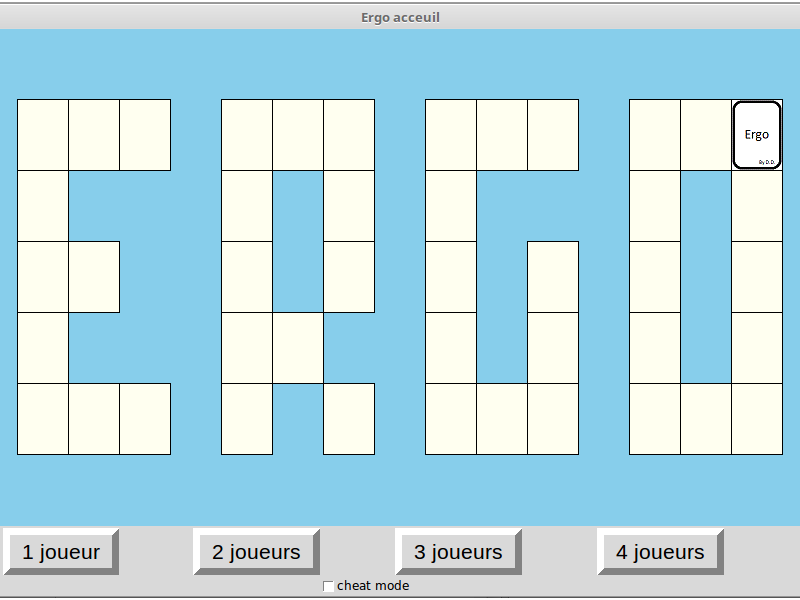
\includegraphics[scale=0.35]{../images/ima1.png}
\end{center}
\caption{Fenêtre d'introduction}
\label{ergoIntro}
\end{figure} 

Elle permet de créer une fenêtre d’accueil avec une animation au démarrage. La méthode animate\_letter permet de simuler une distribution des cartes suivant la forme des lettres du nom du jeu ERGO.

Quatre boutons permettent d'accéder au jeu dans le mode choisi, et une case à cocher permet de choisir le \og cheat mode \fg. Ce dernier ajoute un bouton \texttt{cheat} à l'interface de jeu qui permet de savoir quels sont les joueurs actuellement démontrés.

Le résultat est visible Figure \ref{GI}.

\subsubsection{outils}

Comme les cartes doivent être placées sur une \og grille \fg{},  deux méthodes \texttt{row\_col2x\_y} et \texttt{x\_y2row\_col} ont été créées pour permettre de passer des coordonnées écran aux coordonnées dans la grille et réciproquement.

Les méthodes \texttt{init\_bind} et \texttt{reset\_bind} permettent de désactiver ou modifier les événements souris à certaines étapes du jeu (pendant l'ouverture de messages ou la sélection des cartes à échanger par \texttt{Revolution}). Dans le cas d'une carte \texttt{Revolution}, la méthode \texttt{select\_revolution} permet de choisir les deux cartes à échanger.

\subsubsection{La méthode drop}

Elle permet de placer la carte sélectionnée par \texttt{select} au bon endroit. Dans le cas d'une carte \og simple \fg, elle doit gérer les cas où on lâche la carte :

\begin{itemize}
\item ldans les prémisses. La carte est alors insérée à la positon choisie dans la preuve;
\item dans la pile. La carte est alors ajoutée à l'attribut \texttt{pile} qui permet éventuellement de la récupérer;
\item dans la zone des mains. La carte est alors remise dans la main du joueur.
\end{itemize}


Différents cas particuliers sont à gérer pour les cartes spéciales :
\begin{itemize}
\item les cartes \texttt{fallacy} et \texttt{Justification} jouées dans la zone des mains. L'attribut \texttt{fallacy} de la classe \texttt{Main} est mis à jour en fonction ;
\item la carte \texttt{Tabula Rasa}. Un message informe de l'effacement qui peut être annulé en appuyant sur la touche Echap;
\item la carte \texttt{revolution}. Un message invite à sélectionner les cartes à échanger;
\item les cartes joker. Une liste à puce permet de sélectionner la carte voulue;
\item la carte \texttt{Ergo}. Si toutes les lettres ont été jouées, met fin à la manche en appelant la méthode \texttt{fin\_manche} de la classe \texttt{Main}.
\end{itemize}

\begin{figure}
\begin{center}
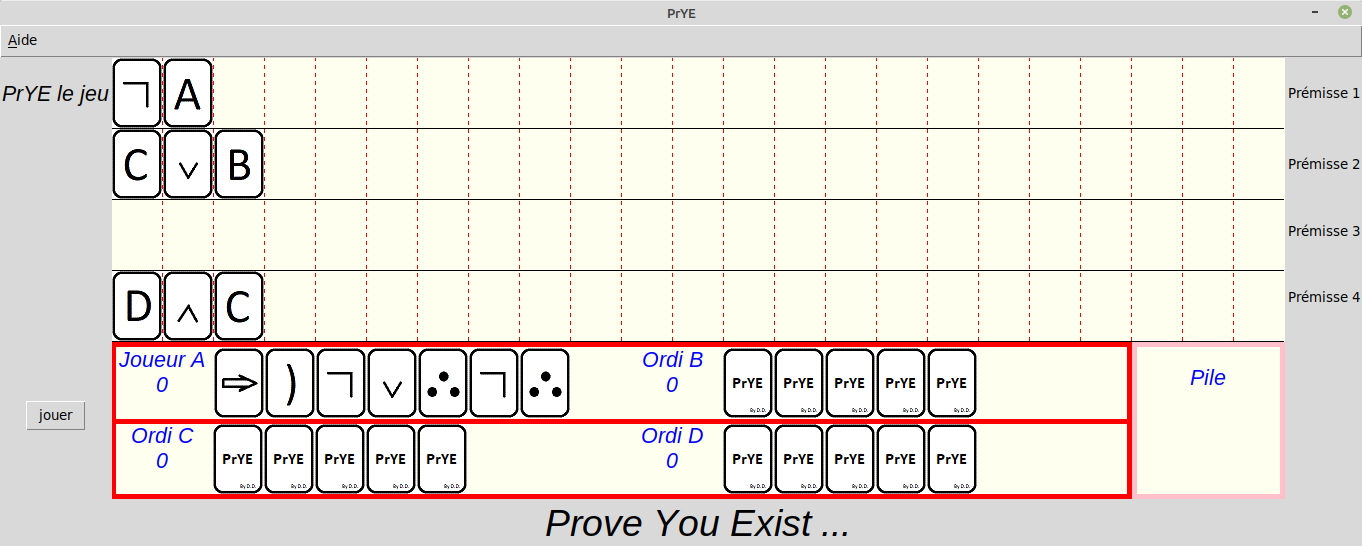
\includegraphics[scale=.35]{../images/ima2.png}
\end{center}
\caption{Rendu final}
\label{GI}
\end{figure}

\subsection{La classe Main}

La classe \texttt{Main} gère le jeu en lui même. C'est elle qui gère l'initialisation du jeu, le passage d'un tour au suivant et la fin de partie. Elle utilise la classe \texttt{ErgoCanvas} pour la gestion du canvas, la classe \texttt{Deck} pour le jeu de carte, les classes \texttt{Proof} et \texttt{Demonstration} (implémentée par \texttt{ForceBrute} ou \texttt{DPLL}) pour la gestion de la preuve et la classe \texttt{Ordi} (implémentée par \texttt{OrdiRandom} ou \texttt{OrdiScore}) pour le jeu de l'ordinateur. 

Les règles du jeu sont dans un fichier html associé à un fichier css . Elles sont affichées dans le navigateur par défaut grâce au module \texttt{webbrowser}. On y trouve les détails d'utilisation des cartes spéciales, les règles de logique et quelques captures d'écran.


\section{Algorithmes utilisés}

\subsection{Passage en notation polonaise inversée : algorithme Shunting-yard}

Une des premier problème algorithmique a été de transformer l'écriture algébrique des preuves en une notation plus utilisable. Ayant pas mal travaillé avec mes élèves sur l'évaluation d'une expression en notation polonaise inversée (NPI), je me disais que je devrais arriver à quelque chose si je pouvais transformer l'écriture algébrique en NPI. J'ai fait quelques recherches la dessus, et je suis tombé sur l'algorithme de \href{https://fr.wikipedia.org/wiki/Algorithme_Shunting-yard}{Shunting-yard}.

Je l'ai légèrement adapté au contexte (proposition logique au lieu de d'expression mathématique) pour obtenir l'algorithme \ref{Shunting-yard}.


\begin{algorithm}[h]
\caption{Algorithme de passage en notation polonaise inversée}
\label{Shunting-yard}
\Entree{Une liste \texttt{input} de cartes (propositions ou connecteurs)}
\Sortie{Une liste npi correspondant a la notation polonaise inversée de l'entrée}
\Trait{
Créer une \texttt{pile} vide\;
\texttt{npi} $\leftarrow []$ \;
\PourCh{\texttt{carte} de \texttt{input}}{
	\uSi{\texttt{carte} est une lettre}{ajouter \texttt{carte} à \texttt{npi}}
	\uSinonSi{\texttt{carte} est un parenthèse ouvrante}{empiler \texttt{carte}}
	\uSinonSi{\texttt{carte} est une parenthèse fermante}{
		\Tq{pile est non vide et que le sommet de la pile n'est pas une parenthèse ouvrante}{dépiler une carte et l'ajouter à \texttt{npi}}
		\eSi{pile est vide}{quitter \tcp*[l]{Problème de parenthésage}}{dépiler la parenthèse ouvrante}
		}
	\Sinon{
		\Tq{pile est non vide et que le sommet de la pile a une priorité supérieure à \texttt{carte}}{dépiler une carte et l'ajouter à \texttt{npi}}
		empiler \texttt{carte}
		}
	}
\Tq{pile est non vide}{
	dépiler une carte et l'ajouter à \texttt{npi}\;
	\Si{la carte est une parenthèse ouvrante}{quitter \tcp*[l]{Problème de parenthésage}}
	}
}
\end{algorithm}

\subsection{Évaluation de la preuve}

\subsubsection{Force brute}

Ici, mon idée a été d'attaquer le problème en force brute : tester tous les modèles possible (comme il y a 4 variables, il y a seulement $2^4=16$ possibilités) et pour chacun évaluer la preuve. Si le résultat est Vrai, c'est que le modèle est admissible et on le mémorise. Ensuite, on regarde pour chaque variable si elle a toujours la même valeur (Vrai ou Faux) dans tous les modèles admissibles. Si c'est la cas, la variable est prouvée ou niée.

Pour l'évaluation d'une formule, j'ai utilisé l'algorithme classique d'évaluation d'une expression en NPI (algorithme \ref{evalNPI}).

\begin{algorithm}[h]
\caption{Algorithme d'évaluation d'une formule}
\label{evalNPI}
\Entrees{Une liste \texttt{npi} de carte en NPI et une interprétation}
\Sortie{L'évaluation de la liste}
\Trait{
Créer une pile vide\;
\PourCh{\texttt{carte} de \texttt{npi}}{
	\uSi{\texttt{carte} est une lettre}{empiler sa valeur dans l'interprétation}
	\uSinonSi{\texttt{carte} est un opérateur binaire}{
		dépiler les deux dernières valeurs\;
		effectuer l'opération entre ces valeurs\;
		empiler le résultat
		}
	\Sinon(\tcp*[h]{c'est un opérateur unaire, le NON}){
		dépiler la dernière valeur\;
		empiler sa négation
		}
	}
\Retour{le sommet de \texttt{pile}} \tcp*[l]{qui ne doit avoir qu'un élément}
}
\end{algorithm}

\subsubsection{Algorithme de Davis-Putnam-Logemann-Loveland (DPLL)}

Même si l'algorithme précédent marche bien dans le contexte qui nous intéresse (4 variables propositionnelles), comme l'algorithme DPLL (algorithme \ref{algoDPLL}) nous a été présenté dans le cours de logique, j'ai voulu l'implémenter. Pour cela, il fallait commencer par transformer la preuve au format NPI en une Forme Conjonctive Normale (FCN) sous forme d'une liste de clauses. Cela se fait en 4 étapes :
\begin{itemize}
\item élimination des implications ($A \implies B \equiv \neg A \vee B$) ;
\item utilisation des lois de Morgan ($\neg (A \vee B) \equiv \neg A \wedge \neg B$ et $\neg (A \wedge B) \equiv \neg A \vee \neg B$) ;
\item élimination des doubles négations ($\neg \neg A \equiv A$) ;
\item développement ($A \vee (B \wedge C) \equiv (A \vee B) \wedge (A \vee C)$).
\end{itemize}


\begin{algorithm}[h]
\caption{Algorithme de Davis-Putnam-Logemann-Loveland (DPLL)}
\label{algoDPLL}
\Entrees{Une liste de clauses \texttt{clause\_list} et un modèle partiel \texttt{model}}
\Sortie{Vrai si on peut compléter le modèle partiel en un modèle complet, Faux sinon}
\Trait{
	\Tq{\texttt{clause\_list} contient une clause unitaire \texttt{[lit]}}{
		ajouter la valeur de \texttt{lit} au modèle \;
		supprimer toutes les clauses contenant \texttt{lit} \;
		supprimer $\neg \texttt{lit}$ de toutes les clauses où il apparaît \;
	}
	\lSi{il ne reste plus de clause}{\Retour{Vrai}}
	\lSi{\texttt{clause\_list} contient une clause vide}{\Retour{Faux}}
	\PourCh{variable \texttt{var} non testée}{
		$\texttt{model\_tmp}[\texttt{var}] \leftarrow $ Faux (resp. Vrai)\; 
		\Si(\tcp*[f]{La négation est prouvée}){non DPLL(\texttt{clause\_list}, \texttt{model\_tmp})}{
			$\texttt{model}[\texttt{var}] \leftarrow$ Vrai (resp. Faux) \;
			supprimer toutes les clauses contenant $\neg \texttt{var}$ \;
			supprimer \texttt{var} de toutes les clauses où il apparaît \;
			\Retour{DPLL(\texttt{clause\_list}, \texttt{model})}
		}
	$\texttt{model}[\texttt{var}] \leftarrow None$ \tcp*{\texttt{var} est indécidable}
	}
	\Retour{Vrai} \tcp*{Toutes les variables on été testées}
}

\end{algorithm}

\section{Évolutions possibles}

Les calculs du score dans la classe \texttt{OrdiScore} dépend de plusieurs paramètres. Je pense que le choix de ces paramètres pourrait se prêter assez bien à un algorithme génétique en faisant jouer l'ordinateur contre lui même et en faisant des croisements entre les coups gagnants.

On pourrait aussi tester d'autres méthodes pour le jeu de l'ordinateur. J'avais éventuellement pensé à un minimax en testant toutes les cartes qui n'ont pas encore été jouées, mais je pense que ça va faire trop de calculs.


\appendix

\begin{a3_landscape}
\section{Diagramme des classes}
\vspace*{-1cm}
\input{"diagramme des classes"}
\end{a3_landscape}
\end{document}

